\vspace{-5pt} 
\section{REAL DATA}
\label{sec:real_data}
\vspace{-5pt} 
With a population exceeding $20$ million, Mexico city stands as one of the most dynamic cities in the world, coupled with the rapid urbanization which led to a huge demand for water. The primary source of Mexico City's water supply is aquifers, and heavy water pumping is the main factor causing subsidence and deformation over the city \cite{yan2012mexico}.
We use a stack of $20$ \acs{SAR} images over the Mexico City acquired every $12$ days, from $14$ August $2019$ to $10$ April $2020$, corresponding to $8$ months to assess the performance of the proposed \acs{SMLEPL} approach.
\begin{figure}[!h]
    \centering
    \begin{subfigure}[b]{\columnwidth}
        \centering
        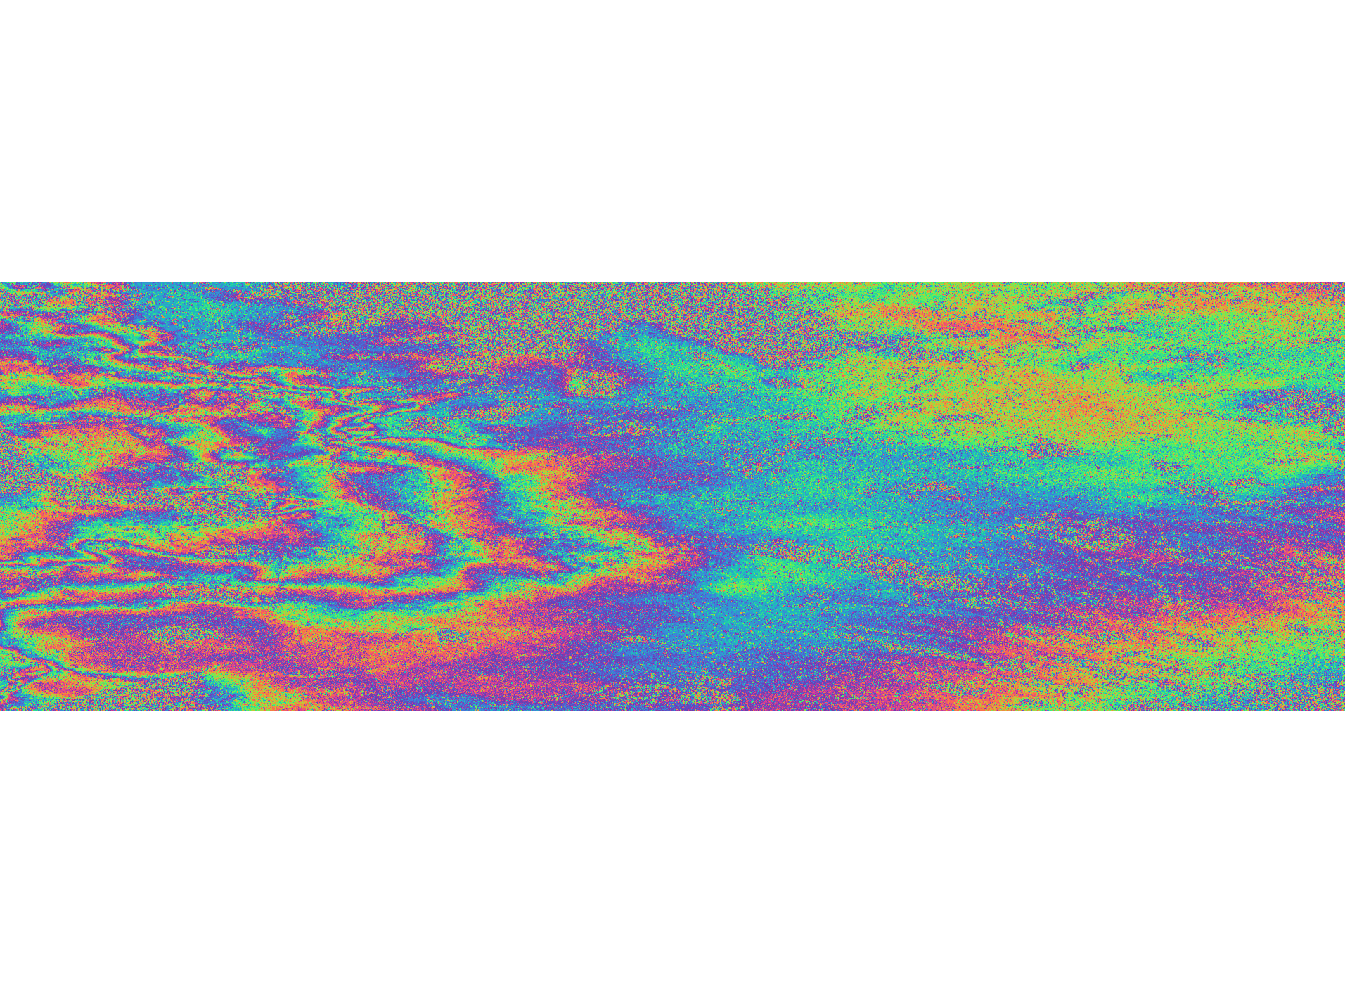
\includegraphics[trim={0 10cm 0 10cm},clip,width=0.7\textwidth]{./imageandplot/phase_GPL_date_20_crop.png}
        \caption{\ac{MLEPL}}
    \end{subfigure}
    \hfill
    \begin{subfigure}[b]{\columnwidth}
        \centering
        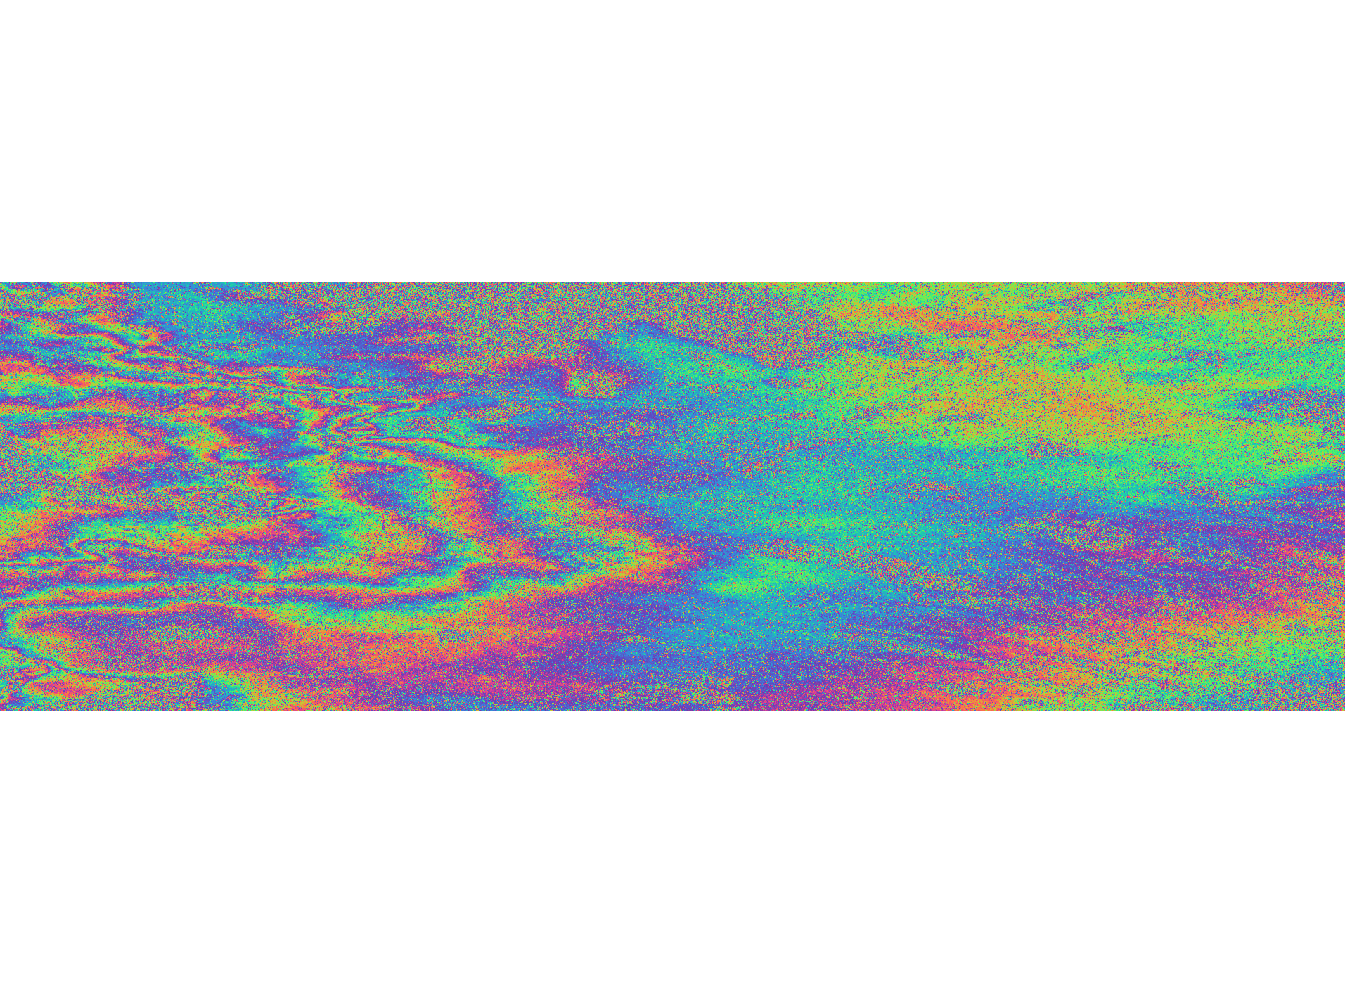
\includegraphics[trim={0 10cm 0 10cm},clip,width=0.7\textwidth]{./imageandplot/phase_sequential_date_20_overlap=4_process=5.png}
        \caption{\acs{SMLEPL}}
    \end{subfigure}
    \hfill
    \begin{subfigure}[b]{\columnwidth}
        \centering
        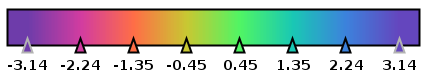
\includegraphics[width=0.6\textwidth, height=2.5em]{./imageandplot/subset_2_of_sequential_date_20_legend.png}
    \end{subfigure}
    \caption{Close-up view of interferograms ($14$ August $2019$ - $10$ April $2020$) estimated by (a) \ac{MLEPL}, and (b) \acs{SMLEPL} in case $l = 20$ and $n = 64$}
    \label{fig:real_data}
\end{figure}
The interferograms estimated by both the \ac{MLEPL} and the proposed \acs{SMLEPL} approach, are illustrated in Fig ~\ref{fig:real_data}. In both cases, the multi-looking window, denoted as $n = 8 \times 8$, remains the same.  The \ac{MLEPL} and \acs{SMLEPL} methods yield the same results, however the sequential approach demonstrates significantly faster execution time than the \acs{MLEPL} when applied to real data.


